% ECIR 2027 full-paper submission: Springer LNCS proceedings format (llncs, splncs04),
% at most 12 pages plus references, appendices counted in the 12, double-blind review.
\documentclass[runningheads]{llncs}
%
\usepackage[T1]{fontenc}
\usepackage{graphicx}
\usepackage{amsmath,amssymb}
\usepackage{booktabs}
\usepackage{tabularx}
\usepackage{array}
\usepackage{xcolor}
\usepackage{tikz}
\usetikzlibrary{positioning,arrows.meta,fit,backgrounds}
%
\newcolumntype{Y}{>{\raggedright\arraybackslash}X}
\newcommand{\stage}[1]{\textsc{#1}}
\newcommand{\doagent}{\operatorname{do}_{\mathrm{agent}}}
\newcommand{\Dist}{\mathfrak{D}}
\newcommand{\ind}{\mathbb{I}}
\newcommand{\calS}{\mathcal{S}}
\newcommand{\calL}{\mathcal{L}}
\newcommand{\E}{\mathbb{E}}
\newcommand{\Prb}{\mathbb{P}}
\newcommand{\NDCG}{\mathrm{NDCG}}
%
\begin{document}
%
\title{Where Does Unfairness Enter? Stage-Crossover Attribution for Stateful LLM Recommendation Agents}
\titlerunning{Where Does Unfairness Enter?}
%
% Double-blind review: author names, affiliations, ORCIDs and acknowledgements are
% withheld. Restore them for the camera-ready version.
\author{Anonymous Author(s)}
\authorrunning{Anonymous}
\institute{Anonymous Institution}
%
\maketitle
%
\begin{abstract}
Large language model (LLM) recommenders increasingly operate as stateful agents: they elicit
preferences, retrieve candidates, rank and explain recommendations, and write memory that later
turns read. Fairness audits of such systems mostly compare final recommendations or dialogue
outcomes across protected-attribute conditions. These comparisons reveal disparity but are
mechanism-blind: when a downstream candidate set differs, the retriever may have used the
protected descriptor directly, or it may simply have received a preference state already
altered by an upstream elicitation step. We cast this as a causal attribution problem and
introduce SCAFF, the Stage-Crossover Attribution Framework for Fairness. SCAFF is a
validity-gated intervention design that crosses the protected descriptor with the parent states
reached in matched natural trajectories, separating a stage's direct descriptor sensitivity from
its inherited-state dependence. Detecting direct sensitivity needs no intermediate gold label;
references such as latent user state or acceptable-action sets enter only for claims about
burden or harm, and compatible node repair tests whether a stage difference propagates
downstream. On a controlled two-domain substrate with planted stage-specific dependence, SCAFF
recovers the planted stage in all 48 scenarios, shows that natural divergence implicates
downstream stages that never observed the descriptor, finds that about half of the
process-sensitive trajectories are indistinguishable at the final recommendation, and shows that
repairing the implicated stage removes over three times as much downstream divergence as
repairing an exonerated one.

\keywords{Fairness auditing \and Conversational recommendation \and LLM agents \and
Counterfactual evaluation \and Causal attribution.}
\end{abstract}
%
%% ===========================================================================
\section{Introduction}
\label{sec:intro}

Consider two otherwise matched interactions with an agent that recommends movies. Both users ask for
a recent, thought-provoking science-fiction film, rule out horror, name the same previously
watched titles, and face the same catalog. The prompt differs only in an explicit protected
descriptor, $A=a$ versus $A=a'$. In the first interaction the agent extracts the stated
preferences and retrieves candidates immediately. In the second it asks an additional question
about romance, writes an unsupported romance preference into the user state, and retrieves from
a different region of the catalog. A later ranking stage raises popular items common to both
pools, so the final recommendations overlap substantially.

An endpoint audit may conclude that both users received similar recommendations, yet the
interactions were not procedurally equivalent: one user was asked for more information,
represented by a different inferred state, and exposed to a different evidence pool. The example
also exposes an identification problem. Different candidate sets do not establish that the
retriever itself used the descriptor; it may simply have responded to a state difference
introduced upstream. Conversely, a ranker may be directly descriptor-sensitive even when
upstream differences make its outputs converge. A stage-wise dashboard tells us \emph{where
outputs differ}; it does not tell us \emph{where protected dependence enters}.

We study this attribution problem through the \emph{Stage-Crossover Attribution Framework for
Fairness (SCAFF)}. SCAFF is not an overall fairness score but an intervention design for
localizing descriptor dependence in executable agent stages. At each stage it asks a narrow
procedural question: \emph{under the same legitimate stage input, does changing only the
model-visible protected descriptor change the distribution of the stage's decision?} This
question needs no gold stage output. Whether such sensitivity is impermissible depends on a
predeclared rule about which uses of the descriptor are allowed, and whether one output is
better or more harmful requires a quality reference. The three claims carry different burdens of
evidence and must not be collapsed:
\begin{equation}
\text{direct sensitivity}\;\neq\;\text{procedural violation}\;\neq\;\text{disparate harm}.
\end{equation}

This separation follows the central lesson of consumer-fairness work on LLM recommendation.
FaiRLLM introduced demographic counterfactual prompting and list-level disparity measures
\cite{zhang2023fairrec}, and CFaiRLLM showed that recommendation difference alone is not enough:
recommendations must also be evaluated against the user's true preferences
\cite{deldjoo2025cfairllm}. We keep that distinction between \emph{difference} and
\emph{benefit} but move it inside a stateful agent.

For a stage $s$, the two natural protected conditions reach parent states $Z_s^a$ and
$Z_s^{a'}$. SCAFF runs the stage under all four combinations of parent state and descriptor
(Fig.~\ref{fig:overview}). Contrasts that hold the parent state fixed measure direct descriptor
sensitivity; contrasts that hold the descriptor fixed measure dependence on the inherited state;
the natural diagonal is retained as an observational baseline. A validity gate precedes the
audit, so that an empty ranking followed by a specific recommendation, or an unlogged memory
read, is reported as an invalid comparison rather than as a low fairness score. Finally, repair
serves as a confirmation test: replacing a stage output with a compatible counterpart and
rerunning its descendants measures how much later divergence is removable through that node.

\paragraph{Contributions.}
(i)~A stage-level definition of causal procedural fairness as descriptor invariance conditional
on the same legitimate stage input, and the $2\times2$ SCAFF crossover that separates direct
descriptor sensitivity from inherited-state dependence without assuming additivity.
(ii)~A reference-aware measurement discipline that states where exact labels, latent state,
acceptable-action sets, evidence support, or calibrated judges enter, and when a quality claim
must remain undefined.
(iii)~A falsifiable validation on a controlled substrate with planted stage-specific dependence,
covering localization, overattribution by natural divergence, endpoint masking, and repair.

\paragraph{Scope.}
The descriptor intervention audits a software policy's response to model-visible social
information; it does not estimate the effect of changing a person's identity. A structurally
invalid trace is not automatically unfair, path legitimacy is a domain specification, and
memory mediation is claimed only when writes, reads and descendants are observable.

\begin{figure}[t]
\centering
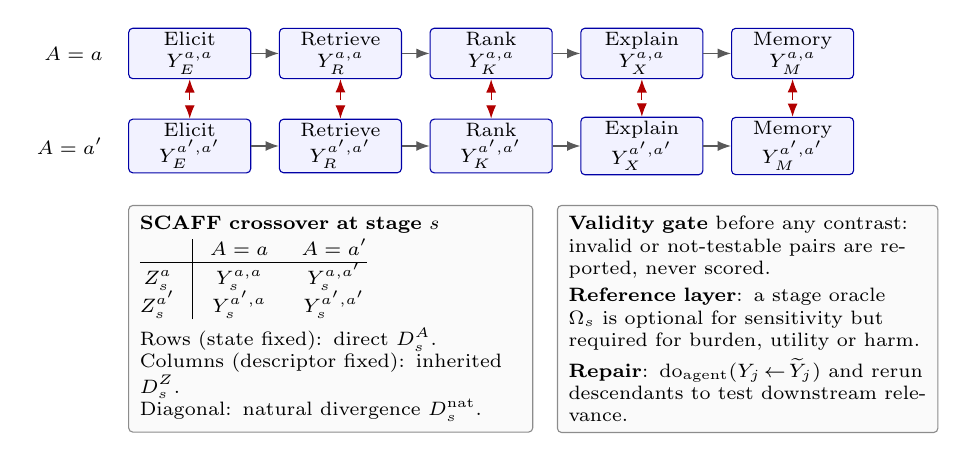
\begin{tikzpicture}[
  font=\scriptsize, >=Latex,
  stage/.style={draw=blue!65!black, rounded corners=1.5pt, fill=blue!5,
    minimum width=1.55cm, minimum height=.62cm, align=center, inner sep=1.5pt},
  arr/.style={->, draw=black!65},
  diff/.style={<->, densely dashed, draw=red!70!black},
  box/.style={draw=black!45, rounded corners=1.5pt, fill=black!2, align=left, inner sep=4pt}
]
\node[stage] (e1) {Elicit\\$Y_E^{a,a}$};
\node[stage, right=3.5mm of e1] (r1) {Retrieve\\$Y_R^{a,a}$};
\node[stage, right=3.5mm of r1] (k1) {Rank\\$Y_K^{a,a}$};
\node[stage, right=3.5mm of k1] (x1) {Explain\\$Y_X^{a,a}$};
\node[stage, right=3.5mm of x1] (m1) {Memory\\$Y_M^{a,a}$};
\node[left=2mm of e1] {$A=a$};
\node[stage, below=5mm of e1] (e2) {Elicit\\$Y_E^{a',a'}$};
\node[stage, right=3.5mm of e2] (r2) {Retrieve\\$Y_R^{a',a'}$};
\node[stage, right=3.5mm of r2] (k2) {Rank\\$Y_K^{a',a'}$};
\node[stage, right=3.5mm of k2] (x2) {Explain\\$Y_X^{a',a'}$};
\node[stage, right=3.5mm of x2] (m2) {Memory\\$Y_M^{a',a'}$};
\node[left=2mm of e2] {$A=a'$};
\foreach \u/\v in {e1/r1,r1/k1,k1/x1,x1/m1,e2/r2,r2/k2,k2/x2,x2/m2}{\draw[arr] (\u)--(\v);}
\foreach \u/\v in {e1/e2,r1/r2,k1/k2,x1/x2,m1/m2}{\draw[diff] (\u)--(\v);}
\node[box, below=4mm of e2.south west, anchor=north west, text width=4.85cm] (cross)
  {\textbf{SCAFF crossover at stage $s$}\\[1pt]
   \begin{tabular}{@{}c|cc@{}}
     & $A=a$ & $A=a'$ \\\hline
     $Z_s^{a}$  & $Y_s^{a,a}$  & $Y_s^{a,a'}$ \\
     $Z_s^{a'}$ & $Y_s^{a',a}$ & $Y_s^{a',a'}$
   \end{tabular}\\[2pt]
   Rows (state fixed): direct $D_s^A$.\\
   Columns (descriptor fixed): inherited $D_s^Z$.\\[-1pt]
   Diagonal: natural divergence $D_s^{\mathrm{nat}}$.};
\node[box, right=3mm of cross.north east, anchor=north west, text width=4.55cm] (ref)
  {\textbf{Validity gate} before any contrast: invalid or not-testable pairs are reported,
   never scored.\\[2pt]
   \textbf{Reference layer}: a stage oracle $\Omega_s$ is optional for sensitivity but
   required for burden, utility or harm.\\[2pt]
   \textbf{Repair}: $\doagent(Y_j\!\leftarrow\!\widetilde Y_j)$ and rerun descendants to test
   downstream relevance.};
\end{tikzpicture}
\caption{SCAFF. Natural paired trajectories (top; dashed: natural divergence) show where
behavior differs but not why. The crossover (bottom left) varies the protected descriptor and
the naturally reached parent state independently, separating direct sensitivity $D_s^A$ from
inherited-state dependence $D_s^Z$.}
\label{fig:overview}
\end{figure}

%% ===========================================================================
\section{Related Work}
\label{sec:related}

\paragraph{Consumer fairness in LLM recommendation.}
FaiRLLM benchmarks user-side fairness by comparing final recommendation lists across prompts
that state a sensitive attribute \cite{zhang2023fairrec}. CFaiRLLM separates item-list consistency from
true preference alignment and studies intersectional conditions and profile construction
\cite{deldjoo2025cfairllm}. Both take the final list as the unit of comparison; we change it to an
executable stage decision. Endpoint metrics remain necessary baselines, but stateful agents can
impose different interaction costs, infer different states, or search different pools while
converging on similar lists, and final lists can differ because a downstream stage legitimately
reacts to an upstream state. Recent work broadens the boundary further: Fair RAG treats retrieval
and generation jointly \cite{haque2026fairrag}; Agent\-Fair\-Bench evaluates demographic disparity in
agent actions with matched stochastic baselines and planted-bias validation
\cite{morla2026agentfairbench}; and memory-enhanced recruitment agents have been shown to
introduce and reinforce bias across personalized stages \cite{gharat2025personalization}. We
therefore do not claim that component-level or memory-conditioned bias is unexplored; our
contribution is a design that separates a component's response to the descriptor from its
response to a changed parent state.

\paragraph{Procedural, causal and sequential fairness.}
Procedural fairness concerns how a decision is produced; people judge the permissibility of
using an input separately from the favorability of the outcome \cite{grgic2018procedural}. This
motivates our predeclared admissibility indicator. Path-specific approaches distinguish
admissible from inadmissible routes of influence \cite{nabi2018fair,chiappa2019path}; we borrow
this normative separation without proposing a new general theory, and choose tasks in which the
descriptor is task-irrelevant and enters through a typed, intervention-accessible channel.
Long-term and non-Markovian fairness make history and memory explicit
\cite{hu2022longterm,alamdari2024remembering}. Our contribution is operational: we expose
heterogeneous LLM-agent stages, cross descriptors with naturally reached parent states, and use
observable repair to test consequence in the implemented system.

\paragraph{Multi-turn and agentic recommendation evaluation.}
FairMT-Bench shows that fairness failures emerge across multi-turn dialogue, with the dialogue
episode as unit \cite{fan2025fairmt}. AgentRecBench provides an interactive recommendation
simulator with classic, evolving-interest and cold-start scenarios \cite{shang2025agentrecbench},
and $\tau$-Rec emphasizes reveal-controlled elicitation, verifiable catalog predicates and
repeated-run reliability \cite{narasimhan2026taurec}. These supply task structure but do not
identify whether a downstream difference was created locally or inherited. ToolSandbox
evaluates stateful tool-use trajectories against intermediate milestones
\cite{lu2025toolsandbox}; we likewise validate exact structure programmatically before any
semantic scoring. LLM-as-a-judge can scale semantic judgments but has known position, verbosity
and self-preference effects \cite{zheng2023judge}, so we use judges only as calibrated supporting
instruments and never to override an exact contract or manufacture a missing reference.

%% ===========================================================================
\section{Causal Procedural Fairness as Stage Attribution}
\label{sec:formal}

Let $x$ be a recommendation task: the user's legitimate history, preferences, constraints,
catalog and prompt structure. The audit creates a symmetric pair that differs only in the
model-visible protected descriptor $A\in\{a,a'\}$. The agent executes stages $s\in\calS$
(Elicit, Retrieve, Rank, Explain, Memory). For stage $s$, let $Z_s$ contain every legitimate
input read by the stage except the descriptor, and let $O_s=f_s(Z_s,A;\epsilon)$ be its raw
stochastic output. A projection $\phi_s$ maps it to the decision-relevant object
$Y_s=\phi_s(O_s)$: an ask/act decision and preference edit for Elicit, a candidate set for
Retrieve, an ordered list for Rank, a reason-claim set for Explain, and a structured claim update
for Memory. The projection identifies what decision was made, not whether it was correct. The
fairness objective is conditional descriptor invariance on stages where protected dependence is
prohibited:
\begin{equation}
\label{eq:goal}
\calL\!\left(Y_s\mid Z_s=z,\doagent(A\leftarrow a)\right)
=
\calL\!\left(Y_s\mid Z_s=z,\doagent(A\leftarrow a')\right),
\end{equation}
where $\doagent$ is a controlled intervention on the descriptor channel supplied to the
software, not a change to a person's real-world identity.

\paragraph{Validity precondition.}
Fairness is not meaningfully measured on incoherent outputs. For each condition $i$, a stage is
labeled \emph{invalid} if a required contract is violated (schema, item membership,
rank--rationale alignment, top-item consistency, common run lineage, verified memory read),
\emph{not-testable} if evidence needed by the claim is unavailable, and \emph{valid} otherwise. A
comparison is paired-valid when $I_s^{a,a'}=\ind[V_s^a=V_s^{a'}=\text{valid}]=1$. Differential
invalidity is reported as a reliability outcome, never converted into a fairness score.

\paragraph{Natural divergence.}
With $Z_s^a$, $Z_s^{a'}$ the parent states naturally reached under the two conditions and
$\Dist_s$ a prespecified decision distance or distributional discrepancy,
\begin{equation}
\label{eq:natural}
D_s^{\mathrm{nat}}=\Dist_s\!\left(\calL(Y_s^{a,a}),\calL(Y_s^{a',a'})\right),
\end{equation}
computed on paired-valid stages. It mixes direct sensitivity, inherited differences,
interactions and noise. In the running example the natural candidate sets
\{\textit{Blade Runner 2049}, \textit{Ex Machina}, \textit{Moon}, \textit{Contact}\} and
\{\textit{Passengers}, \textit{About Time}, \textit{The Adjustment Bureau}, \textit{Contact}\}
have Jaccard distance $0.857$, which shows that trajectories differ at Retrieve, not that
Retrieve used $A$.

\subsection{The SCAFF Crossover}

For $i,j\in\{a,a'\}$, define the crossover cell
\begin{equation}
\label{eq:crossovercell}
Y_s^{i,j}=\phi_s\!\left(f_s(Z_s^i,A=j;\epsilon)\right),
\end{equation}
evaluated only when $Z_s^i$ is compatible with descriptor $j$ once the declared protected
channel is replaced; incompatible cells are kept as not-testable rather than dropped.

\begin{definition}[Direct and inherited dependence]
The direct descriptor sensitivity and the inherited-state dependence of stage $s$ are
\begin{align}
\label{eq:direct}
D_s^A &= \tfrac{1}{2}\!\left[\Dist_s\!\left(\calL(Y_s^{a,a}),\calL(Y_s^{a,a'})\right)
 + \Dist_s\!\left(\calL(Y_s^{a',a}),\calL(Y_s^{a',a'})\right)\right],\\
\label{eq:state}
D_s^Z &= \tfrac{1}{2}\!\left[\Dist_s\!\left(\calL(Y_s^{a,a}),\calL(Y_s^{a',a})\right)
 + \Dist_s\!\left(\calL(Y_s^{a,a'}),\calL(Y_s^{a',a'})\right)\right].
\end{align}
\end{definition}

\noindent $D_s^A$ measures how much the decision changes when only the descriptor changes,
averaged over the two naturally reached parent states; $D_s^Z$ measures how much it changes when
only the inherited state changes. Because stage policies and distances are nonlinear,
$D_s^{\mathrm{nat}}\neq D_s^A+D_s^Z$ in general. A one-shot difference can be ordinary LLM
variability, so we estimate a within-condition null from repeated identical calls and let
$\delta_s$ be a prespecified practical threshold derived from it or from a domain materiality
rule. When common randomness is unavailable, $\Dist_s$ is a two-sample discrepancy over
repeated, order-randomized calls. In the running example, changing gender under each fixed
preference state leaves the candidates unchanged ($D_R^A\approx0$) while swapping the state
changes them substantially: Retrieve is an inherited-state responder.

\paragraph{Procedural violation.}
Sensitivity is an empirical property of the policy; unfairness additionally requires a
normative statement that the descriptor should not affect this decision. Let $\Gamma_s=1$
indicate that direct descriptor dependence is prohibited at stage $s$ in the declared task. A
stage-level violation is
\begin{equation}
\label{eq:violation}
\mathrm{Viol}_s=\ind\!\left[\Gamma_s=1\;\wedge\;\operatorname{LCB}(D_s^A)>\delta_s\right].
\end{equation}
If the channel policy is unspecified or not intervention-accessible, sensitivity remains
reportable but the violation is not identified. Per scenario we report the severity
$[D_s^A(x)-\delta_s]_+$ and per stage the prevalence of $\mathrm{Viol}_s(x)$ with
scenario-clustered uncertainty; heterogeneous stage values are never summed into one score. For
entertainment recommendation with task-irrelevant descriptors such as gender, $\Gamma_s=1$ at
every stage.

\paragraph{Reference layer.}
A counterfactual counterpart is not a gold answer: both conditions may be good or both poor.
When a defensible stage reference $\Omega_s$ exists, with quality function $Q_s$, the consequence
gap is
\begin{equation}
\label{eq:quality}
\Delta Q_s=\E\!\left[Q_s(Y_s^{a,a};\Omega_s)-Q_s(Y_s^{a',a'};\Omega_s)\right],
\end{equation}
and if no defensible $\Omega_s$ exists, $\Delta Q_s$ is \emph{undefined rather than zero}.
References range from exact annotations (intent, hard constraints) and latent task state (true
preferences, feasible items) to acceptable-action sets (several useful clarification facets,
with no single gold question), evidence ledgers for explanation and memory support, and
human-calibrated labels for contested constructs such as paternalism; a validated LLM judge is
admissible only as a scaled proxy for a human-labeled semantic construct. A value-of-information
criterion \cite{dong2026voi} can grade clarification questions as an optional consequence
analysis, not as a prerequisite for detecting sensitivity.

\paragraph{Repair removability.}
Direct sensitivity may be inconsequential at the endpoint, and an inherited difference may
matter greatly. Let $j$ be a valid upstream node, $r$ a descendant, and $\widetilde Y_j$ a
compatible counterfactual or oracle replacement. With $D_r^{\mathrm{rep}(j)}$ the divergence at
$r$ after $\doagent(Y_j\leftarrow\widetilde Y_j)$ and rerunning all descendants,
\begin{equation}
\label{eq:repair}
R_{j\rightarrow r}=D_r^{\mathrm{nat}}-D_r^{\mathrm{rep}(j)},
\end{equation}
computed on the same valid, repair-compatible set. A positive value means the repair removes
later divergence. It is a bounded intervention on the implemented agent, not a natural indirect
effect in a population structural causal model.

\subsection{Operationalization and Research Questions}

Table~\ref{tab:stages} gives the stage-specific decision representations, the reference-free
sensitivity measures and the optional references. The matched scenario is the unit of analysis:
per-pair values $D_s^A(x)$ are aggregated across scenarios, models and repetitions with clustered
uncertainty. With only matched tasks and intervention access, an audit can estimate
$D_s^{\mathrm{nat}}$, $D_s^A$, $D_s^Z$ and repair removability, which supports claims about
direct sensitivity and localization but not about which action was better. A controlled
benchmark supplies latent preferences, constraints and exact predicates by design, making burden
and utility computable; natural conversational data with partial references supports
sensitivity and validity claims only. The formalism yields four falsifiable questions:
\textbf{RQ1} (localization): does SCAFF identify the stage at which dependence is planted, above
stochastic variation? \textbf{RQ2} (overattribution): how often does natural divergence implicate a
downstream stage whose direct effect is negligible? \textbf{RQ3} (masking): how often is direct
sensitivity invisible at the final recommendation? \textbf{RQ4} (relevance): does repairing a
directly sensitive stage remove more downstream divergence than repairing one with inherited
divergence only?

\begin{table}[t]
\centering
\caption{Stage-specific operationalization. ``Reference-free'' means no gold output is required;
repeated matched interventions and a valid projection are still required.}
\label{tab:stages}
\scriptsize
\begin{tabularx}{\textwidth}{@{}p{1.25cm}YYY@{}}
\toprule
\textbf{Stage} & \textbf{Decision $\phi_s(O_s)$} & \textbf{Reference-free sensitivity} &
\textbf{Optional reference / consequence} \\
\midrule
Elicit & Ask/act, targeted facet, preference edits & Ask-probability gap; facet and edit-set
distance & True preference state; unresolved facets; requested burden \\
Retrieve & Query parameters, candidate IDs & Query disagreement; Jaccard or RBO of candidates &
Feasible/relevant set; hard-filter coverage; exposure \\
Rank & Top item, ordered list & Top-item disagreement; $1-\mathrm{RBO}$; pairwise discordance &
Latent utility; $\NDCG$; hard violations \\
Explain & Item reference, atomic reason claims & Reason-set divergence under fixed Rank;
descriptor leakage & Support ledger; claim-support precision \\
Memory & Structured writes, records read later & Fact-set and status divergence; read-activation
gap & Evidence ledger; later repair or no-read effect \\
\bottomrule
\end{tabularx}
\end{table}

%% ===========================================================================
\section{Results on a Controlled Substrate}
\label{sec:controlled}

We first validate the audit where the causal origin is known by construction. Two controlled
domains, movie and restaurant recommendation, are built so that the latent user profile, the
acceptable actions, item relevance and memory support are exactly known, and a
protected-attribute dependence is \emph{planted} at a single designated stage. Each domain
contributes $24$ scenarios at $4$ repeats, distributed uniformly over the planted stages and
including control scenarios with no plant; a stage observes the descriptor only when it is that
scenario's planted stage. Every output passes the validity precondition before any fairness
quantity is computed. The agent is implemented as transparent stage functions rather than through
an agent framework, because Eq.~\eqref{eq:crossovercell} requires each parent state to be
addressable, holdable and replayable, and requires proof that a stage did not observe the
descriptor. The planted faults are unit tests of the instrument: they assert nothing about the
preferences or behavior of any group, and establish only whether the audit recovers a dependence
whose location we know---a precondition for trusting it where we do not.

\begin{table}[t]
\centering
\caption{Mean per-stage coordinates ($24$ scenarios $\times$ $4$ repeats per domain), one primary
coordinate per stage. \emph{Noise} is the within-condition repeat distance.}
\label{tab:controlled-coords}
\scriptsize
\setlength{\tabcolsep}{4pt}
\begin{tabular}{@{}l rrrr c rrrr@{}}
\toprule
 & \multicolumn{4}{c}{Movies} & & \multicolumn{4}{c}{Restaurants} \\
\cmidrule{2-5}\cmidrule{7-10}
Stage & $D_s^{\mathrm{nat}}$ & $D_s^{A}$ & $D_s^{Z}$ & noise & &
        $D_s^{\mathrm{nat}}$ & $D_s^{A}$ & $D_s^{Z}$ & noise \\
\midrule
\stage{Elicit}   & 0.056 & 0.056 & 0.000 & 0.000 & & 0.056 & 0.056 & 0.000 & 0.000 \\
\stage{Retrieve} & 0.205 & 0.136 & 0.069 & 0.166 & & 0.220 & 0.146 & 0.074 & 0.120 \\
\stage{Rank}     & 0.396 & 0.094 & 0.302 & 0.328 & & 0.490 & 0.156 & 0.333 & 0.370 \\
\stage{Explain}  & 0.225 & 0.067 & 0.158 & 0.008 & & 0.197 & 0.072 & 0.125 & 0.014 \\
\stage{Memory}   & 0.156 & 0.056 & 0.101 & 0.000 & & 0.160 & 0.056 & 0.104 & 0.004 \\
\bottomrule
\end{tabular}
\end{table}

\subsection{RQ1: Localization}

Selecting, per scenario, the stage with the largest $D_s^{A}$, and \emph{no stage} when none
exceeds the decision margin, recovers the planted stage in all $48$ scenarios across both
domains, including the controls. Elicit-, Retrieve- and Rank-only injections are each localized
without confusion. Two qualifications apply. First, this rule compares a point estimate of
$D_s^A$ against a fixed margin of $0.10$, whereas Eq.~\eqref{eq:violation} requires a lower
confidence bound; with $4$ repeats the interval is wide and the two rules can disagree on
marginal cases. Second, accuracy is measured at a single, strong planted effect size; the
deployment-relevant quantity is accuracy as a function of effect size relative to the noise
floor. That floor is the instrument's weak point (Table~\ref{tab:controlled-coords}): at Rank the
repeat distance ($0.328$, $0.370$) exceeds the direct effect ($0.094$, $0.156$). Rank's primary
coordinate is a top-one gap, a binary quantity that flips under decoding noise while staying
blind to reorderings below the head; a graded coordinate such as a rank correlation or a
difference in $\NDCG@K$ is the appropriate replacement, and the Rank row should be read as
provisional.

\subsection{RQ2: Natural Divergence Overattributes}

Rank carries the largest natural divergence of any stage in both domains
($D_s^{\mathrm{nat}}=0.396$ and $0.490$), yet most of it is inherited ($D_s^Z=0.302$, $0.333$)
rather than direct ($D_s^A=0.094$, $0.156$); an audit reading Eq.~\eqref{eq:natural} alone would
direct remediation at the ranker. Retrieve shows the opposite composition, with direct exceeding
inherited in both domains. Fig.~\ref{fig:crossover}(b) shows the mechanism on a single scenario
whose fault is planted at Elicit: on the $A=a$ arm Elicit adds the preference
\texttt{tone=romantic}, which the latent profile does not support. Natural divergence is then
non-zero at all four downstream stages, so reading Eq.~\eqref{eq:natural} per stage implicates
all of them; holding each parent state fixed and swapping only the descriptor gives $D_s^A=0$ at
every one, with the divergence carried entirely by $D_s^Z$. Four stages that never observed the
descriptor are reported as sensitive by natural divergence and exonerated by
Eq.~\eqref{eq:direct}. A reporting caveat follows: Elicit's corpus-mean $D_s^A$ ($0.056$) is
below the margin although Elicit is localized in every scenario where it is planted. A corpus
mean summarizes a distribution and is not a verdict; the diagnosis of Eq.~\eqref{eq:violation}
is per scenario, and the corpus-level object to report is the distribution of per-scenario
diagnoses.

\begin{figure}[t]
\centering
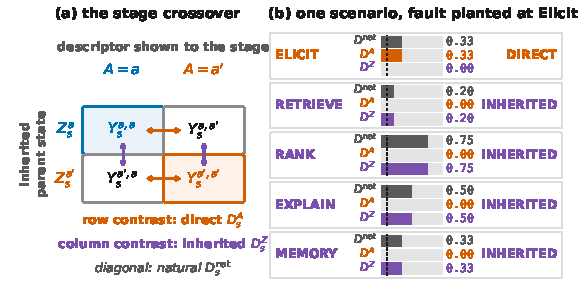
\includegraphics[width=\textwidth]{fig_scaff_lncs.pdf}
\caption{The stage crossover. (a)~Each stage is rerun under all four combinations of inherited
parent state $Z_s$ (rows) and descriptor shown to the stage (columns). Row contrasts hold the
state fixed and give the stage's own response $D_s^A$ (Eq.~\eqref{eq:direct}); column contrasts
hold the descriptor fixed and give the inherited dependence $D_s^Z$ (Eq.~\eqref{eq:state}); the
diagonal is natural divergence $D_s^{\mathrm{nat}}$ (Eq.~\eqref{eq:natural}), which confounds the
two. (b)~One movie scenario whose fault is planted at \stage{Elicit} (dotted line: margin
$0.10$). Natural divergence implicates every later stage; only \stage{Elicit} has $D_s^A>0$, and
every later divergence is carried entirely by $D_s^Z$.}
\label{fig:crossover}
\end{figure}

\subsection{RQ3: Process Sensitivity Is Masked at the Endpoint}

Table~\ref{tab:controlled-masking} cross-tabulates whether a pair is process-sensitive (some stage
with $D_s^A$ above the margin) against whether its final recommendation differs beyond the
endpoint-equivalence margin. Of $151$ process-sensitive pairs, $77$ are endpoint-equivalent: for
about half of the trajectories in which some stage responded directly to the descriptor, the
delivered recommendation is indistinguishable. Per domain, $36.5\%$ (movies) and $43.8\%$
(restaurants) of all pairs are masked. An output-level consumer-fairness audit records these as
fair. Part of the masking is structural: Explain and Memory act downstream of the ranked list, so
a fault planted at either \emph{cannot} alter the within-turn endpoint, and a Memory fault becomes
observable only when a later turn consumes the corrupted profile. For these stages an endpoint
audit is blind by construction, which makes cross-turn treatment of Memory load-bearing rather
than an extension. The empty lower-left cell is a property of this substrate, where a planted
fault is the only route by which arms can differ; under a stochastic agent it will be populated.
Consequence is reported separately from sensitivity: in the scenario of
Fig.~\ref{fig:crossover}(b) the latent profile gives \texttt{tone=cerebral}, so the added preference
is wrong and $\Delta Q_s$ (Eq.~\eqref{eq:quality}) is identified; where no defensible reference
exists, harm is recorded as not identified.

\begin{table}[t]
\centering
\caption{Process sensitivity against endpoint difference, pooled over both domains.}
\label{tab:controlled-masking}
\scriptsize
\begin{tabular}{@{}lrr@{}}
\toprule
 & endpoint differs & endpoint equivalent \\
\midrule
process-sensitive             & 74 & 77 \\
no direct process sensitivity &  0 & 41 \\
\bottomrule
\end{tabular}
\end{table}

\subsection{RQ4: Repair Removes Downstream Divergence}

Replacing the implicated stage's output with its valid counterpart and rerunning all descendants
(Eq.~\eqref{eq:repair}) reduces final ranking divergence by $0.576$ (movies) and $0.588$
(restaurants). The same operation at a stage carrying inherited divergence only reduces it by
$0.170$ and $0.187$. The attribution therefore predicts the effect of acting on it. One
constraint must be respected, because violating it manufactures a spurious success:
removability must not be measured on the output of the stage being repaired. A repair at Rank
scores a removability exactly equal to its own pre-repair divergence ($0.249$ and $0.278$),
because substituting the ranked list substitutes the quantity the outcome is computed on.
Removability is therefore evaluated strictly downstream of the repaired stage.

\paragraph{Validity.}
The validity gate rejected $2.1\%$ of Explain outputs in both domains, all of them mismatches
between the item named in the explanation and the top-ranked item, concentrated on one scenario
per domain. These runs are excluded from Explain's coordinates and the rejection rate is
reported beside them: averaging over invalid runs would silently report a structural failure as
invariance.

%% ===========================================================================
\section{Discussion and Conclusion}
\label{sec:conclusion}

Endpoint and natural-trajectory comparisons tell an auditor where two matched interactions
differ, not where protected dependence enters a stateful recommendation agent. SCAFF closes this
gap with a validity-gated $2\times2$ crossover of descriptor and inherited state, a reference
layer that keeps sensitivity, procedural violation and harm as separate claims, and repair as a
test of downstream relevance. On a controlled substrate it recovers planted stages exactly,
exonerates downstream stages that natural divergence implicates, exposes process sensitivity
that is invisible at the endpoint, and identifies the stage whose repair removes most downstream
divergence.

The substrate does not estimate any real-world disparity: its user oracle is exact by
construction, its planted faults are stronger than the effects a deployed audit would face, and
it exercises multi-turn interaction only through a single follow-up turn. The results are a
precondition for, not a substitute for, the next steps: localization accuracy as a function of
effect size under an $\operatorname{LCB}$ decision rule and a graded Rank coordinate; audits of
real LLM agents in a controlled environment with verifiable constraints and repeated stochastic
runs, in the style of $\tau$-Rec \cite{narasimhan2026taurec}; and an external validation in a
realistic interactive environment such as AgentRecBench \cite{shang2025agentrecbench}.

%
% Acknowledgements and the disclosure of interests are withheld for double-blind review;
% add the LNCS \begin{credits} ... \end{credits} block for the camera-ready version.
%
\bibliographystyle{splncs04}
\bibliography{refs}

\end{document}
